\subsection {Программная платформа и язык программирования}
Для решения поставленной задачи необходимо использовать функциональную, эффективную и удобную платформу для разработки. В качестве такой платформы была выбрана среда разработки Qt Creator.
Qt - это кросс-платформенная библиотека C++ классов для создания графических пользовательских интерфейсов (GUI) от фирмы Digia. Эта библиотека полностью объектно-ориентированная, что обеспечивает лёгкое расширение возможностей и создание новых компонентов. Ко всему прочему, она поддерживает огромнейшее количество платформ.

Qt позволяет запускать написанное с его помощью ПО в большинстве современных операционных систем путём простой компиляции программы для каждой ОС без изменения исходного кода. Включает в себя все основные классы, которые могут потребоваться при разработке прикладного программного обеспечения, начиная от элементов графического интерфейса и заканчивая классами для работы с изображениями, видео и мультипоточными приложениями. Qt является полностью объектно-ориентированным, легко расширяемым и поддерживающим технику компонентного программирования.

Список использованных классов фреймворка Qt:
\begin{itemize}
\item QDebug;
\item QDir;
\item QFile;
\item QTextStream;
\item QSrting;
\item *QImage;
\item QTime.
\end{itemize}

Класс QDebug обеспечивает выходной поток для отладочной информации.

Класс QDir обеспечивает доступ к структуре каталогов и их содержимого.

Класс QFile предоставляет интерфейс для чтения и записи файлов.

Класс QTextStream предоставляет удобный интерфейс для чтения и записи текста.

Класс QString обеспечивает строку символов Unicode.

Класс QImage предоставляет аппаратно-независимую работу с изображениями, даёт прямой доступ к данным каждого пикселя, и может быть использован в качестве устройства рисования. На ранних стадиях создание ПО это класс использовался в качестве основного инструмента для работы с изображениями, но впоследствии при переходе на основные модули библиотеки DV стал использовался объект Data2D, и методы работы с ними.

Класс QTime обеспечивает функции таймера. В проекте используется для оценки быстродействия разрабатываемого модуля при разных входных параметрах~\cite{qt}.

Для совместимости с библиотекой DV, решено использовать систему сборки CMake, взамен QMake. CMake широко используется с Qt.
Список классов и методов библиотеки DV используемых в проекте:
\begin{itemize}
\item Data2D;
\item Matx22d;
\item Vec2d;
\item VF2d.
\end{itemize}

Список стандартных библиотек используемых в проекте:

\begin{itemize}
\item getopt.h;
\item iostream;
\item math.h;
\item stdlib.h;
\item vector.
\end{itemize}

getopt библиотечная функция, специально разработанная для того чтобы облегчить обработку входных команд. 

iostream заголовочный файл с классами, функциями и переменными для организации ввода-вывода в языке программирования C++. Он включён в стандартную библиотеку C++. Название образовано от Input/Output Stream (``поток ввода-вывода'').

math.h — заголовочный файл стандартной библиотеки языка программирования С, разработанный для выполнения простых математических операций.

stdlib.h — заголовочный файл стандартной библиотеки языка Си, который содержит в себе функции, занимающиеся выделением памяти, контроль процесса выполнения программы, преобразования типов и другие.

vector.h — это замена стандартному динамическому массиву, память для которого выделяется вручную, с помощью оператора new.
\subsection {Контроль версий}
Система контроля версий (СКВ) — это система, регистрирующая изменения в одном или нескольких файлах с тем, чтобы в дальнейшем была возможность вернуться к определённым старым версиям этих файлов.

Для разработки программного комплекса решено использовать Git.

Git  — распределённая система управления версиями файлов. Проект был создан Линусом Торвальдсом для управления разработкой ядра Linux, как противоположность системе управления версиями Subversion (также известная как «SVN») \cite{progit}.

Преимущества использования системы версий, очевидны:
\begin{itemize}
\item возможность возвращать к прежнему состоянию отдельные файлы или весь проект;
%\item возможность создавать свои ветки, не мешая при этом другим разработчикам;
\item возможность удалённой работы с текстами программ;
\item доступ к последним изменениям в коде, т.к. всё хранятся на сервере github.com;
\item тексты программ открыты, доступ к ним можно получить доступ в интернет;
%\item удобство работы с tex документами;
\item просматривать происходящие со временем изменения.
\end{itemize}

Основные постулаты работы в системе Git:
\begin{itemize}
\item каждая задача решается в своей ветке;
\item сохраняем изменения сразу, как что-то получили осмысленное;
%\item в master мержится не разработчиком, а вторым человеком, который производит вычитку и тестирование изменения;
\item все сохранённые изменения должны быть осмысленно подписаны/прокомментированы.
\end{itemize}
\begin{figure}[ht]
\center{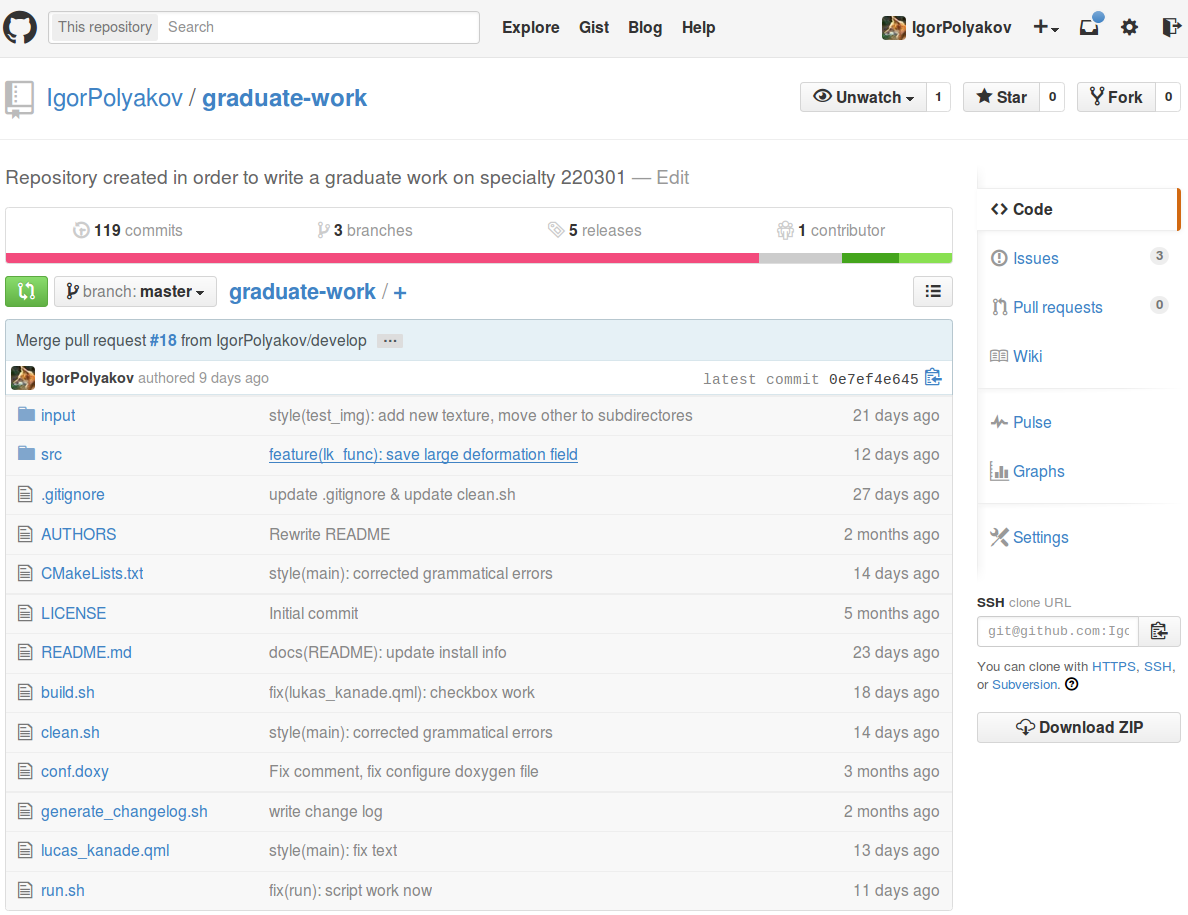
\includegraphics[width=0.9\linewidth]{github}}
\caption{Тексты программ в репозитории github}
\label{pic:github}
\end{figure}

Для работы над проектом был использован репозиторий на сервере github.com. Слепок последних изменений из репозитория можно взять по адресу: git clone git@github.com:IgorPolyakov/graduate-work.git


\subsection{Описание консольного интерфейса программы}% (выбор цветовой палитры экранных форм, расположение элементов управления на них, использование «горячих» клавиш  акселераторов, выпадающих меню и пр.)}
Интерфейс программы представлен в двух реализациях.
Первый — консольная программа в стиле классического Unix. Интерфейс командной строки более гибкий, позволяет выставить необходимые опции/флаги и запустить программу. Особенности в сравнении с графическим интерфейсом:
\begin{itemize}
\item Интерфейс командной строки позволяет писать скрипты для автоматизации запуска и тестирования с различными входными параметрами, что средствами графического интерфейса гораздо сложнее;
\item Большая функциональность;
\item Некая сложность при использовании, неопытным пользователям;
\item Невозможность просмотра выходных результатов.
\end{itemize}

\begin{figure}[ht]
\center{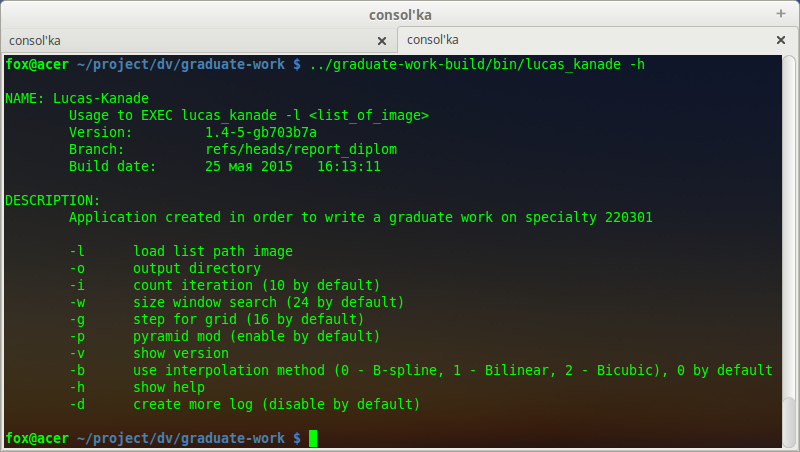
\includegraphics[width=0.8\linewidth]{consol_screen}}
\caption{Пример консольного интерфейса в среде Linux}
\label{pic:con_scr}
\end{figure}

\subsubsection{Перечень команд для запуска}
\begin{itemize}
\item l — список изображений для обработки;
\item o — директория для выходных результатов;
\item i — число уточнений при поиске смещённой части (по умолчанию равна 10);
\item w — радиус окна поиска (по умолчанию равна 24);
\item g — шаг между векторами оптического потока(по умолчанию равна 16);
\item p — применить метод пирамиды(по умолчанию опция включена);
\item v — показать версию программного обеспечения;
\item b — использование метода интерполяции(0 — Б-сплайн, 1 — Билинейная, 2 — Бикубическая), по умолчанию 0;
\item h — показать краткую справку;
\item d — генерировать подробный лог файл(по умолчанию опция выключена).
\end{itemize}
\subsection{Описание графического интерфейса программы}
Второй графический — более удобный для неопытного пользователя. 

\begin{figure}[ht]
\center{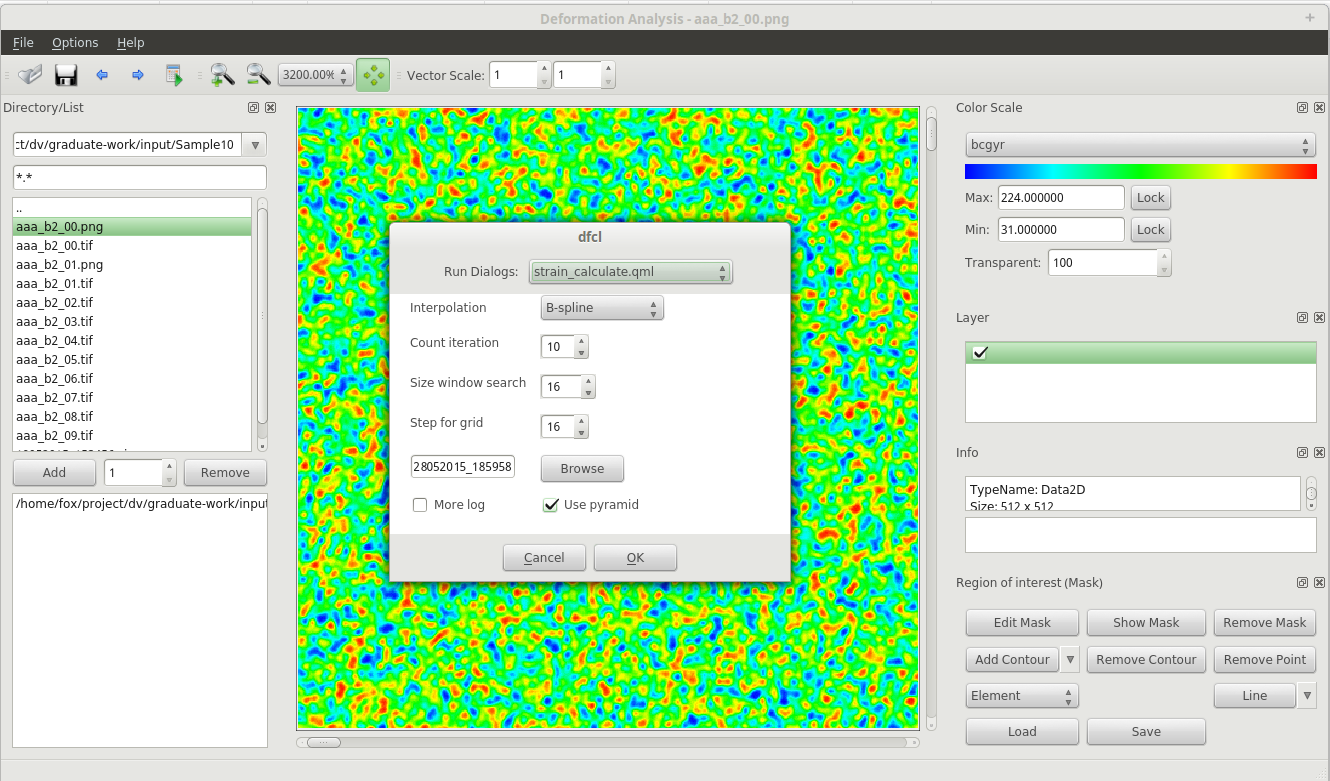
\includegraphics[width=0.8\linewidth]{gui_screen}}
\caption{Пример графического интерфейса}
\label{pic:gui_scr}
\end{figure}

\subsection{Справочную систему пользователя для разрабатываемого модуля,требования к уровню квалификации пользователя}
\subsection{Листинг программы с комментариями, поясняющими работу основных блоков}
\subsection{Блок схему оригинальных, разработанных автором, алгоритмов работы основных, по мнению автора, программных модулей}
\subsection{Тестовый пример для контроля адекватного функционирования разработанного программного модуля и протокол (листинг) результатов работы программы на этом тестовом примере}